\section{最小生成樹}
    \subsection{概念}
    最小生成樹常常用在處理道路規劃問題,雖然我們沒有直接的看見他在生活中
    的應用,但是肯定有,而且競賽常常會考喔。

    那什麼是最小生成樹?就是這個樹的邊集$\in$圖的邊集合的子集,所有這樣的集合中
    ,邊權總和最小的那一個。

    同樣的,兩種演算法的概念並不相同,所以就讓我分別講解吧。

    \subsection{Kruskal}

    \textbf{概念}

    我們盡可能加入權重最小的邊,如果加入後會產生環就不加,就這樣跑完所有的邊
    就會找到最小生成樹了。

    判斷會不會產生環需要DSU,把加入的邊a,b兩端所屬的連通分量合併,
    這恰好是並查集最擅長的操作。

    排序會是複雜度最高的操作,因此時間複雜度為$O(m\log{(n)})$。

    \textbf{實作}

\begin{lstlisting}[caption=Kruskal算法]
struct edge{
    int f,t,w;
};
bool operator<(edge a,edge b){
    return a.w<b.w;
}

int dsu[10010],rk[10010];
void init(int n){
    for(int i=0;i<=n;i++){
        dsu[i]=i;
        rk[i]=1;
    }
}

int find(int a){
    if(dsu[a]==a)
        return a;
    return find(dsu[a]);
}

bool same(int a,int b){
    return find(a)==find(b);
}

void uni(int a,int b){
    if(rk[find(a)]==rk[find(b)]){
        dsu[find(b)]=dsu[find(a)];
        rk[a]++;
    }else if(rk[find(a)]>rk[find(b)]){
        dsu[find(b)]=dsu[find(a)];
    }else{
        dsu[find(a)]=dsu[find(b)];
    }
}

int main(){
    // input
        
    sort(g.begin(),g.end());
        
    int ans=0,ct=0;
        
    init(n);
    for(auto e:g){
        if(!same(e.f,e.t)){
            uni(e.f,e.t);
            ct++;
            ans+=e.w;
        }
    }
}
\end{lstlisting}

    \subsection{Prim}

    因為我沒有用過Prim,而且兩者的時間複雜度同為$O(m\log{(n)})$。

    不過還是稍微介紹一下概念。他有點像Dijkstra,不過是每次都把
    距離已經確定的點集合最近的邊加入。

    如圖,下一個頂點為距離D或A最近的頂點。B距D為9,距A為7,E距D為15,
    F距D為6。因此,F距D或A最近,因此將頂點F與相應邊DF圖上比較亮的顏色。

    \begin{figure}[ht]
        \centering
        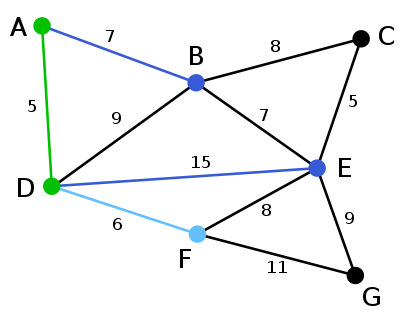
\includegraphics[width=0.5\textwidth]{../Images/Graph4.png}
    \end{figure}

    我們同樣可以利用\verb|priority_queue|提升效率,所以同樣是$O(m\log{(n)})$。

    \subsection{範例與練習}

    \problem Sprout OJ 734 模板題

    \problem 洛谷P1194 買禮物

    \textbf{題目敘述}

    又到了一年一度的明明生日了,明明想要買 $B$ 樣東西,巧的是,這 $B$ 樣東西價格都是 $A$ 元。

    但是,商店老闆說最近有促銷活動,也就是:如果你買了第 $I$ 樣東西,再買第 $J$ 樣,
    那麼就可以只花 $K_{I,J}$ 元,更巧的是,$K_{I,J}$ 竟然等於 $K_{J,I}$。

    現在明明想知道,他最少要花多少錢。

    \textbf{輸入說明}

    第一行兩個整數,$A,B$。

    接下來 $B$ 行,每行 $B$ 個數,第 $I$ 行第 $J$ 個為 $K_{I,J}$。

    我們保證 $K_{I,J}=K_{J,I}$ 並且 $K_{I,I}=0$。

    特別的,如果 $K_{I,J}=0$,那麼表示這兩樣東西之間不會導致優惠。

    $1\le B\le500,0\le A,K_{I,J}\le1000$

    \textbf{輸出說明}

    一個整數,為最小要花的錢數。

    \textbf{範例測試}

    \begin{tabular}{|m{7cm}|m{7cm}|}
        \hline
        範例輸入 1 & 範例輸出 1 \\
        \hline
        \verb|3 3| & \verb|7| \\
        \verb|0 2 4| & \\
        \verb|2 0 2| & \\
        \verb|4 2 0| & \\
        \hline
    \end{tabular}

    \problem 洛谷P1396 營救

    \textbf{題目敘述}

    ``咚咚咚……",``查水表!"原來是查水表來了,現在哪裡找這麼熱心上門的查表員啊!
    小明感動得熱淚盈眶,開起了門$\cdots$

    媽媽下班回家,街坊鄰居說小明被一群陌生人強行押上了警車!媽媽豐富的經驗告訴她小明被帶到了 
    $t$ 區,而自己在 $s$ 區。

    該市有 $m$ 條大道連接 $n$ 個區,一條大道將兩個區相連接,每個大道有一個擁擠度。
    小明的媽媽雖然很著急,但是不願意擁擠的人潮衝亂了她優雅的步伐。所以請你幫她規劃一條從
     $s$ 至 $t$ 的路線,使得經過道路的擁擠度最大值最小。

    \textbf{輸入說明}

    第一行有四個用空格隔開的 $n$,$m$,$s$,$t$,其含義見【題目敘述】。

    接下來 $m$ 行,每行三個整數 $u, v, w$,表示有一條大道連接區 $u$ 和區 $v$,
    且擁擠度為 $w$。

    $1 \leq n\leq 10^4$,$1 \leq m \leq 2 \times 10^4$,$w \leq 10^4$,
    $1 \leq s, t \leq n$。且從 $s$ 出發一定能到達 $t$

    \textbf{輸出說明}

    輸出一行一個整數,代表最大的擁擠度。

    \textbf{範例測試}

    \begin{tabular}{|m{7cm}|m{7cm}|}
        \hline
        範例輸入 1 & 範例輸出 1 \\
        \hline
        \verb|3 3 1 3| & \verb|2| \\
        \verb|1 2 2| & \\
        \verb|2 3 1| & \\
        \verb|1 3 3| & \\
        \hline
    \end{tabular}